\subsection{Applying Masks to an Image}
\label{sect:mask}

In this problem, you will write a function that will apply a ``mask''
to an image. The core of this transformation is this function:
\begin{quote}
\begin{lstlisting}
int[] apply_mask(pixel_t[] pixels, int width, int height,
                 int[] mask, int maskwidth);
\end{lstlisting}
\end{quote}
The returned array should contain the results of running the mask
computation, a weighted sum, on each pixel in the input.
This is an array of \emph{integers}, not an array of pixels;
each integer in the returned array corresponds to a pixel in the
given image.

\paragraph{Masks}

In addition to an input image, we pass this transformation a
\emph{mask}, an $n \times n$ array of integers
representing \emph{weights}.  For our purposes, $n$ must be
odd. This means that the $n \times n$ array has a well defined center
--- the \emph{origin}. The weights in the mask can be arbitrary integers
--- positive, negative, or zero.

For each pixel in the input image, think of the mask as being placed
on top of the image so its origin is on the pixel we wish to
examine. The intensity value of each pixel under the mask is multiplied by
the corresponding value in the mask that covers it. These products are added
together.  Always use the original values for each pixel for each mask
calculation, not the new values you compute as you process the image.

\begin{figure}
  \begin{minipage}[c]{0.6\textwidth}\centering
    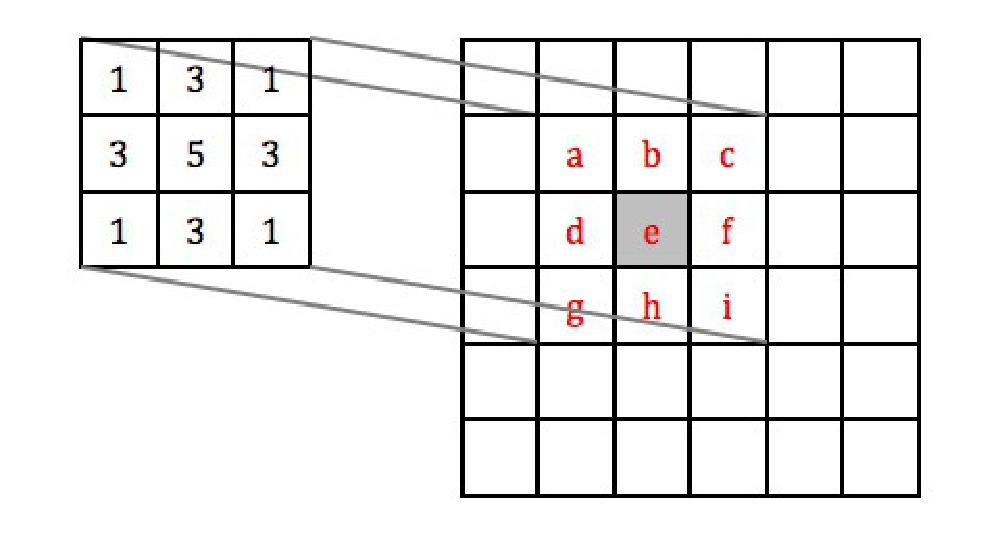
\includegraphics[scale=0.45]{\img/blurexample-eps-converted-to.pdf}
  \end{minipage}\hfill
  \begin{minipage}[c]{0.37\textwidth}
    \caption{Overlay the $3 \times 3$ mask over the image so it is centered on
      pixel $e$ to compute the new value for pixel $e$.}
    \label{fig:blur-example1}
  \end{minipage}
\end{figure}

\begin{figure}
  \begin{minipage}[c]{0.6\textwidth}\centering
    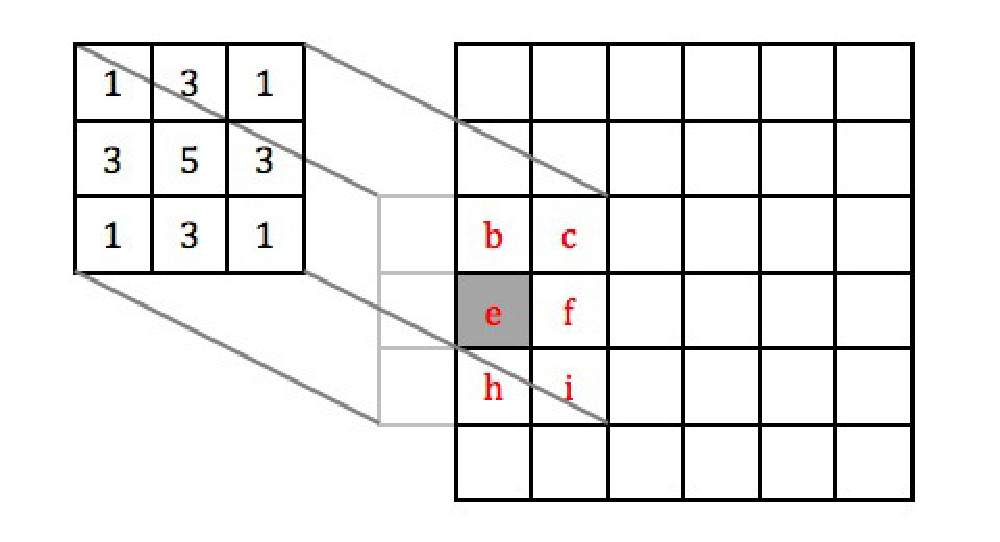
\includegraphics[scale=0.45]{\img/blurexample2-eps-converted-to.pdf}
%% The integer in index 18 of the returned array should be
%% \lstinline'3b + c + 5e + 3f + 3h + i'\\ where \lstinline'b' is the average intensity
%% of the pixel labeled \lstinline'b' and so on.
  \end{minipage}\hfill
  \begin{minipage}[c]{0.37\textwidth}
    \caption{If the mask hangs over the edge of the image, use only those mask
      values that cover the image in the weighted sum.}
    \label{fig:blur-example2}
  \end{minipage}
\end{figure}

For example, refer to Figure~\ref{fig:blur-example1}, which shows a $3
\times 3$ mask and an image that we want to perform the mask
computation on. Suppose we want to compute the result of the mask
computation for pixel \lstinline'e'. This result would be:
\begin{quote}
\begin{lstlisting}
a + 3b + c + 3d + 5e + 3f + g + 3h + i
\end{lstlisting}
\end{quote}
\pagebreak[4] Instead of doing this calculation for each channel
individually, use the average value of the red, green, and blue
channels --- we ignore the alpha channel. Going back to the example in
Figure~\ref{fig:blur-example1}, if the pixels \lstinline'a' and
\lstinline'e' are both given by $(a, r, g, b) = (255, 107, 9, 217)$,
then use $(107 + 9 + 217) / 3 = 111$ as the average intensity of those
pixels. If every other pixel in that figure is given by $(a, r, g, b)
= (15, 200, 120, 100)$ for an average intensity of $140$, then index
14 (which corresponds to pixel \lstinline'e' in
Figure~\ref{fig:blur-example1}) of the returned array should store
$2766$:
\begin{quote}
$111 + (3\times{}140) + 140 + (3\times{}140) + (5\times{}111) + (3\times{}140) + 140 + (3\times{}140) + 140 = 2766$
\end{quote}

Note that sometimes when you center the mask over a pixel you want to operate
on, the mask will hang over the edge of the image. In this case, compute the
weighted sum of only those pixels the mask covers. For the example shown in
Figure~\ref{fig:blur-example2}, the result stored in index 18 of the returned
array, which corresponds to pixel \lstinline'e', is given by
\begin{quote}
\begin{lstlisting}
3b + c + 5e + 3f + 3h + i
\end{lstlisting}
\end{quote}
where \lstinline'b' is the average intensity
of the pixel labeled \lstinline'b' and so on.


\begin{task}[10]
\TAGS{array, safety, testing}
  Create a C0 file \lstinline'mask.c0' implementing a function
  \lstinline'apply_mask'. You may include any auxiliary functions you
  need in the same file, but you should not include a
  \lstinline'main()' function.
\end{task}

You should look at \lstinline'README.txt' to see how to use this
transformation to perform a grayscale blur (\lstinline'maskblur-main.c0')
and edge detection algorithms (\lstinline'maskedge-main.c0'). The next
page talks a little bit about how these algorithms, especially edge
detection, work. You are also strongly encouraged to write some
test cases for your programs in file \lstinline'images-test.c0'.

\begin{figure}[bt]
\centering
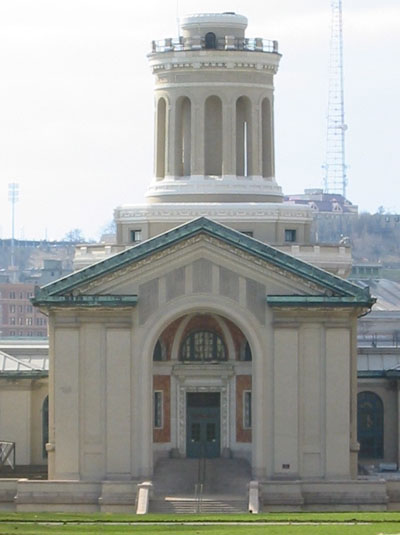
\includegraphics[scale=0.3]{\img/cmu.png}
\quad
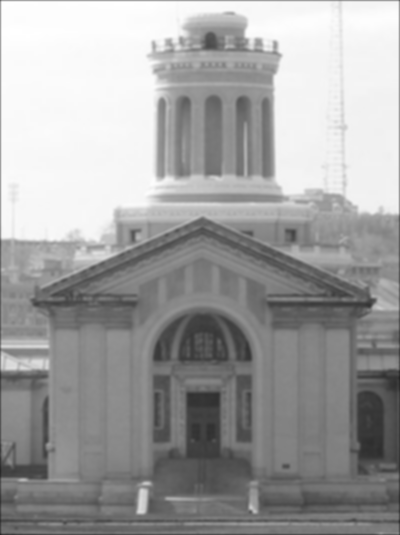
\includegraphics[scale=0.3]{\img/cmu-gaussian.png}
\quad
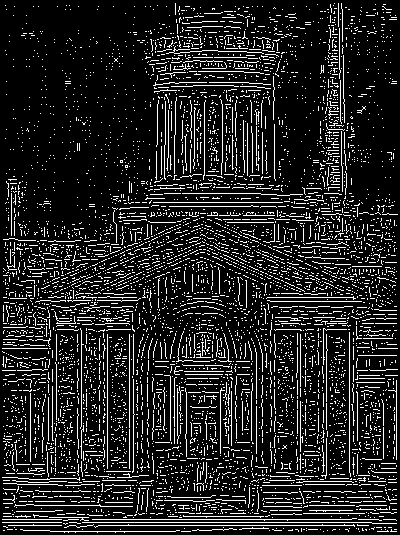
\includegraphics[scale=0.3]{\img/cmu-edge.png}
\caption{Hammerschlag Hall: original image (left), blurred with the mask
  (middle), and after running edge detection (right). See text for mask values.}
\label{fig:carnegie-blur}
\end{figure}

\clearpage
\subsubsection*{Applications}
\label{sect:applications}

The first main function you are given to test your code,
\lstinline'maskblur-main.c0', reads a mask from a text file, specified
by the \lstinline'-m' option. The mask is read in from the file and
passed along to \lstinline'apply_mask'. Then, the data returned from
\lstinline'apply_mask' is used to calculate new intensity values for
the pixels. This is done by summing all of the weights of the mask and
dividing by it. Note that this will cause the edge of the image to
have a lower intensity than it should, since we're not considering the
part of the mask that hangs off of the image, but this is an
acceptable simplification of the problem. Since we're allowing our
masks to have negative values, this creates the possible issue of
having an intensity greater than 255. If this is the case, the
intensities are modified appropriately --- for the blur masks, the
\lstinline'maskblur-main.c0' program will do division to get an
average intensity that is between 0 and 255.  Since we're returning
just one value instead of one per channel, this has the effect of
converting the image to grayscale.

One application of masks is blurring an image, which would be the
effect created by the examples shown in Figure~\ref{fig:blur-example1}
and Figure~\ref{fig:blur-example2}.

The other main function you are given to test your code,
\lstinline'maskedge-main.c0', implements an edge detection algorithm,
which is another application of masks.  The algorithm described here
is an implementation of Canny Edge Detection, using Sobel
operators. In this case, the function \lstinline'apply_mask' is called
three times. The first call will be to blur the image. For this
purpose, the following mask is used:
$$
\left[
\begin{array}{@{}rrrrr@{}}
   2 &  4 &  5 &  4 & 2
\\ 4 &  9 & 12 &  9 & 4
\\ 5 & 12 & 15 & 12 & 5
\\ 4 &  9 & 12 &  9 & 4
\\ 2 &  4 &  5 &  4 & 2
\end{array}
\right]
$$

After getting the resulting grayscale image, two more filters (the Sobel
operators) are applied to it. These filters determine the change in intensity,
which approximates the horizontal and vertical derivatives.
$$
\mathbf{G}_x =
\left[
\begin{array}{@{}rrr@{}}
   -1 & 0 & +1
\\ -2 & 0 & +2
\\ -1 & 0 & +1
\end{array}
\right]
\qquad
\text{and}
\qquad
\mathbf{G}_y =
\left[
\begin{array}{@{}rrr@{}}
   -1 & -2 & -1
\\  0 &  0 &  0
\\ +1 & +2 & +1
\end{array}
\right]
$$

After these two calls to \lstinline'apply_mask', the values obtained
are used to search for edges based on the magnitude and direction of
the change in intensity. An example of the final result is shown in
Figure~\ref{fig:carnegie-blur}.

You can even see the intermediate results of the X and Y filters individually by
trying:
\begin{quote}
\begin{lstlisting}[language={[coin]C}]
./maskblur -i images/cmu.png -m sobelX.txt -o images/cmu-edgeX.png
./maskblur -i images/cmu.png -m sobelY.txt -o images/cmu-edgeY.png
\end{lstlisting}
\end{quote}



%%% Local Variables:
%%% mode: latex
%%% TeX-master: "main"
%%% End:
